
%% bare_conf.tex
%% V1.3
%% 2007/01/11
%% by Michael Shell
%% See:
%% http://www.michaelshell.org/
%% for current contact information.
%%
%% This is a skeleton file demonstrating the use of IEEEtran.cls
%% (requires IEEEtran.cls version 1.7 or later) with an IEEE conference paper.
%%
%% Support sites:
%% http://www.michaelshell.org/tex/ieeetran/
%% http://www.ctan.org/tex-archive/macros/latex/contrib/IEEEtran/
%% and
%% http://www.ieee.org/

%%*************************************************************************
%% Legal Notice:
%% This code is offered as-is without any warranty either expressed or
%% implied; without even the implied warranty of MERCHANTABILITY or
%% FITNESS FOR A PARTICULAR PURPOSE!
%% User assumes all risk.
%% In no event shall IEEE or any contributor to this code be liable for
%% any damages or losses, including, but not limited to, incidental,
%% consequential, or any other damages, resulting from the use or misuse
%% of any information contained here.
%%
%% All comments are the opinions of their respective authors and are not
%% necessarily endorsed by the IEEE.
%%
%% This work is distributed under the LaTeX Project Public License (LPPL)
%% ( http://www.latex-project.org/ ) version 1.3, and may be freely used,
%% distributed and modified. A copy of the LPPL, version 1.3, is included
%% in the base LaTeX documentation of all distributions of LaTeX released
%% 2003/12/01 or later.
%% Retain all contribution notices and credits.
%% ** Modified files should be clearly indicated as such, including  **
%% ** renaming them and changing author support contact information. **
%%
%% File list of work: IEEEtran.cls, IEEEtran_HOWTO.pdf, bare_adv.tex,
%%                    bare_conf.tex, bare_jrnl.tex, bare_jrnl_compsoc.tex
%%*************************************************************************

% *** Authors should verify (and, if needed, correct) their LaTeX system  ***
% *** with the testflow diagnostic prior to trusting their LaTeX platform ***
% *** with production work. IEEE's font choices can trigger bugs that do  ***
% *** not appear when using other class files.                            ***
% The testflow support page is at:
% http://www.michaelshell.org/tex/testflow/



% Note that the a4paper option is mainly intended so that authors in
% countries using A4 can easily print to A4 and see how their papers will
% look in print - the typesetting of the document will not typically be
% affected with changes in paper size (but the bottom and side margins will).
% Use the testflow package mentioned above to verify correct handling of
% both paper sizes by the user's LaTeX system.
%
% Also note that the "draftcls" or "draftclsnofoot", not "draft", option
% should be used if it is desired that the figures are to be displayed in
% draft mode.
%
\documentclass[conference]{IEEEtran}
\usepackage{blindtext, graphicx}
% Add the compsoc option for Computer Society conferences.
%
% If IEEEtran.cls has not been installed into the LaTeX system files,
% manually specify the path to it like:
% \documentclass[conference]{../sty/IEEEtran}





% Some very useful LaTeX packages include:
% (uncomment the ones you want to load)


% *** MISC UTILITY PACKAGES ***
%
%\usepackage{ifpdf}
% Heiko Oberdiek's ifpdf.sty is very useful if you need conditional
% compilation based on whether the output is pdf or dvi.
% usage:
% \ifpdf
%   % pdf code
% \else
%   % dvi code
% \fi
% The latest version of ifpdf.sty can be obtained from:
% http://www.ctan.org/tex-archive/macros/latex/contrib/oberdiek/
% Also, note that IEEEtran.cls V1.7 and later provides a builtin
% \ifCLASSINFOpdf conditional that works the same way.
% When switching from latex to pdflatex and vice-versa, the compiler may
% have to be run twice to clear warning/error messages.






% *** CITATION PACKAGES ***
%
%\usepackage{cite}
% cite.sty was written by Donald Arseneau
% V1.6 and later of IEEEtran pre-defines the format of the cite.sty package
% \cite{} output to follow that of IEEE. Loading the cite package will
% result in citation numbers being automatically sorted and properly
% "compressed/ranged". e.g., [1], [9], [2], [7], [5], [6] without using
% cite.sty will become [1], [2], [5]--[7], [9] using cite.sty. cite.sty's
% \cite will automatically add leading space, if needed. Use cite.sty's
% noadjust option (cite.sty V3.8 and later) if you want to turn this off.
% cite.sty is already installed on most LaTeX systems. Be sure and use
% version 4.0 (2003-05-27) and later if using hyperref.sty. cite.sty does
% not currently provide for hyperlinked citations.
% The latest version can be obtained at:
% http://www.ctan.org/tex-archive/macros/latex/contrib/cite/
% The documentation is contained in the cite.sty file itself.






% *** GRAPHICS RELATED PACKAGES ***
%
\ifCLASSINFOpdf
  % \usepackage[pdftex]{graphicx}
  % declare the path(s) where your graphic files are
  % \graphicspath{{../pdf/}{../jpeg/}}
  % and their extensions so you won't have to specify these with
  % every instance of \includegraphics
  % \DeclareGraphicsExtensions{.pdf,.jpeg,.png}
\else
  % or other class option (dvipsone, dvipdf, if not using dvips). graphicx
  % will default to the driver specified in the system graphics.cfg if no
  % driver is specified.
  % \usepackage[dvips]{graphicx}
  % declare the path(s) where your graphic files are
  % \graphicspath{{../eps/}}
  % and their extensions so you won't have to specify these with
  % every instance of \includegraphics
  % \DeclareGraphicsExtensions{.eps}
\fi
% graphicx was written by David Carlisle and Sebastian Rahtz. It is
% required if you want graphics, photos, etc. graphicx.sty is already
% installed on most LaTeX systems. The latest version and documentation can
% be obtained at:
% http://www.ctan.org/tex-archive/macros/latex/required/graphics/
% Another good source of documentation is "Using Imported Graphics in
% LaTeX2e" by Keith Reckdahl which can be found as epslatex.ps or
% epslatex.pdf at: http://www.ctan.org/tex-archive/info/
%
% latex, and pdflatex in dvi mode, support graphics in encapsulated
% postscript (.eps) format. pdflatex in pdf mode supports graphics
% in .pdf, .jpeg, .png and .mps (metapost) formats. Users should ensure
% that all non-photo figures use a vector format (.eps, .pdf, .mps) and
% not a bitmapped formats (.jpeg, .png). IEEE frowns on bitmapped formats
% which can result in "jaggedy"/blurry rendering of lines and letters as
% well as large increases in file sizes.
%
% You can find documentation about the pdfTeX application at:
% http://www.tug.org/applications/pdftex





% *** MATH PACKAGES ***
%
\usepackage[cmex10]{amsmath}
\usepackage{amssymb}
% A popular package from the American Mathematical Society that provides
% many useful and powerful commands for dealing with mathematics. If using
% it, be sure to load this package with the cmex10 option to ensure that
% only type 1 fonts will utilized at all point sizes. Without this option,
% it is possible that some math symbols, particularly those within
% footnotes, will be rendered in bitmap form which will result in a
% document that can not be IEEE Xplore compliant!
%
% Also, note that the amsmath package sets \interdisplaylinepenalty to 10000
% thus preventing page breaks from occurring within multiline equations. Use:
%\interdisplaylinepenalty=2500
% after loading amsmath to restore such page breaks as IEEEtran.cls normally
% does. amsmath.sty is already installed on most LaTeX systems. The latest
% version and documentation can be obtained at:
% http://www.ctan.org/tex-archive/macros/latex/required/amslatex/math/





% *** SPECIALIZED LIST PACKAGES ***
%
%\usepackage{algorithmic}
% algorithmic.sty was written by Peter Williams and Rogerio Brito.
% This package provides an algorithmic environment fo describing algorithms.
% You can use the algorithmic environment in-text or within a figure
% environment to provide for a floating algorithm. Do NOT use the algorithm
% floating environment provided by algorithm.sty (by the same authors) or
% algorithm2e.sty (by Christophe Fiorio) as IEEE does not use dedicated
% algorithm float types and packages that provide these will not provide
% correct IEEE style captions. The latest version and documentation of
% algorithmic.sty can be obtained at:
% http://www.ctan.org/tex-archive/macros/latex/contrib/algorithms/
% There is also a support site at:
% http://algorithms.berlios.de/index.html
% Also of interest may be the (relatively newer and more customizable)
% algorithmicx.sty package by Szasz Janos:
% http://www.ctan.org/tex-archive/macros/latex/contrib/algorithmicx/




% *** ALIGNMENT PACKAGES ***
%
%\usepackage{array}
% Frank Mittelbach's and David Carlisle's array.sty patches and improves
% the standard LaTeX2e array and tabular environments to provide better
% appearance and additional user controls. As the default LaTeX2e table
% generation code is lacking to the point of almost being broken with
% respect to the quality of the end results, all users are strongly
% advised to use an enhanced (at the very least that provided by array.sty)
% set of table tools. array.sty is already installed on most systems. The
% latest version and documentation can be obtained at:
% http://www.ctan.org/tex-archive/macros/latex/required/tools/


%\usepackage{mdwmath}
%\usepackage{mdwtab}
% Also highly recommended is Mark Wooding's extremely powerful MDW tools,
% especially mdwmath.sty and mdwtab.sty which are used to format equations
% and tables, respectively. The MDWtools set is already installed on most
% LaTeX systems. The lastest version and documentation is available at:
% http://www.ctan.org/tex-archive/macros/latex/contrib/mdwtools/


% IEEEtran contains the IEEEeqnarray family of commands that can be used to
% generate multiline equations as well as matrices, tables, etc., of high
% quality.


%\usepackage{eqparbox}
% Also of notable interest is Scott Pakin's eqparbox package for creating
% (automatically sized) equal width boxes - aka "natural width parboxes".
% Available at:
% http://www.ctan.org/tex-archive/macros/latex/contrib/eqparbox/





% *** SUBFIGURE PACKAGES ***
%\usepackage[tight,footnotesize]{subfigure}
% subfigure.sty was written by Steven Douglas Cochran. This package makes it
% easy to put subfigures in your figures. e.g., "Figure 1a and 1b". For IEEE
% work, it is a good idea to load it with the tight package option to reduce
% the amount of white space around the subfigures. subfigure.sty is already
% installed on most LaTeX systems. The latest version and documentation can
% be obtained at:
% http://www.ctan.org/tex-archive/obsolete/macros/latex/contrib/subfigure/
% subfigure.sty has been superceeded by subfig.sty.



%\usepackage[caption=false]{caption}
%\usepackage[font=footnotesize]{subfig}
% subfig.sty, also written by Steven Douglas Cochran, is the modern
% replacement for subfigure.sty. However, subfig.sty requires and
% automatically loads Axel Sommerfeldt's caption.sty which will override
% IEEEtran.cls handling of captions and this will result in nonIEEE style
% figure/table captions. To prevent this problem, be sure and preload
% caption.sty with its "caption=false" package option. This is will preserve
% IEEEtran.cls handing of captions. Version 1.3 (2005/06/28) and later
% (recommended due to many improvements over 1.2) of subfig.sty supports
% the caption=false option directly:
%\usepackage[caption=false,font=footnotesize]{subfig}
%
% The latest version and documentation can be obtained at:
% http://www.ctan.org/tex-archive/macros/latex/contrib/subfig/
% The latest version and documentation of caption.sty can be obtained at:
% http://www.ctan.org/tex-archive/macros/latex/contrib/caption/




% *** FLOAT PACKAGES ***
%
%\usepackage{fixltx2e}
% fixltx2e, the successor to the earlier fix2col.sty, was written by
% Frank Mittelbach and David Carlisle. This package corrects a few problems
% in the LaTeX2e kernel, the most notable of which is that in current
% LaTeX2e releases, the ordering of single and double column floats is not
% guaranteed to be preserved. Thus, an unpatched LaTeX2e can allow a
% single column figure to be placed prior to an earlier double column
% figure. The latest version and documentation can be found at:
% http://www.ctan.org/tex-archive/macros/latex/base/



%\usepackage{stfloats}
% stfloats.sty was written by Sigitas Tolusis. This package gives LaTeX2e
% the ability to do double column floats at the bottom of the page as well
% as the top. (e.g., "\begin{figure*}[!b]" is not normally possible in
% LaTeX2e). It also provides a command:
%\fnbelowfloat
% to enable the placement of footnotes below bottom floats (the standard
% LaTeX2e kernel puts them above bottom floats). This is an invasive package
% which rewrites many portions of the LaTeX2e float routines. It may not work
% with other packages that modify the LaTeX2e float routines. The latest
% version and documentation can be obtained at:
% http://www.ctan.org/tex-archive/macros/latex/contrib/sttools/
% Documentation is contained in the stfloats.sty comments as well as in the
% presfull.pdf file. Do not use the stfloats baselinefloat ability as IEEE
% does not allow \baselineskip to stretch. Authors submitting work to the
% IEEE should note that IEEE rarely uses double column equations and
% that authors should try to avoid such use. Do not be tempted to use the
% cuted.sty or midfloat.sty packages (also by Sigitas Tolusis) as IEEE does
% not format its papers in such ways.





% *** PDF, URL AND HYPERLINK PACKAGES ***
%
\usepackage{url}
% url.sty was written by Donald Arseneau. It provides better support for
% handling and breaking URLs. url.sty is already installed on most LaTeX
% systems. The latest version can be obtained at:
% http://www.ctan.org/tex-archive/macros/latex/contrib/misc/
% Read the url.sty source comments for usage information. Basically,
% \url{my_url_here}.





% *** Do not adjust lengths that control margins, column widths, etc. ***
% *** Do not use packages that alter fonts (such as pslatex).         ***
% There should be no need to do such things with IEEEtran.cls V1.6 and later.
% (Unless specifically asked to do so by the journal or conference you plan
% to submit to, of course. )


% correct bad hyphenation here
\hyphenation{op-tical net-works semi-conduc-tor}


\begin{document}
%
% paper title
% can use linebreaks \\ within to get better formatting as desired
\title{Bluetooth Low Energy {\textendash} Security issues}


% author names and affiliations
% use a multiple column layout for up to three different
% affiliations
\author{\IEEEauthorblockN{Moritz Schaefer}
\IEEEauthorblockA{School of Electronic Information and\\Electrical Engineering\\
Shanghai Jiao Tong University\\
Email: mollitz@gmail.com}}

% conference papers do not typically use \thanks and this command
% is locked out in conference mode. If really needed, such as for
% the acknowledgment of grants, issue a \IEEEoverridecommandlockouts
% after \documentclass

% for over three affiliations, or if they all won't fit within the width
% of the page, use this alternative format:
%
%\author{\IEEEauthorblockN{Michael Shell\IEEEauthorrefmark{1},
%Homer Simpson\IEEEauthorrefmark{2},
%James Kirk\IEEEauthorrefmark{3},
%Montgomery Scott\IEEEauthorrefmark{3} and
%Eldon Tyrell\IEEEauthorrefmark{4}}
%\IEEEauthorblockA{\IEEEauthorrefmark{1}School of Electrical and Computer Engineering\\
%Georgia Institute of Technology,
%Atlanta, Georgia 30332--0250\\ Email: see http://www.michaelshell.org/contact.html}
%\IEEEauthorblockA{\IEEEauthorrefmark{2}Twentieth Century Fox, Springfield, USA\\
%Email: homer@thesimpsons.com}
%\IEEEauthorblockA{\IEEEauthorrefmark{3}Starfleet Academy, San Francisco, California 96678-2391\\
%Telephone: (800) 555--1212, Fax: (888) 555--1212}
%\IEEEauthorblockA{\IEEEauthorrefmark{4}Tyrell Inc., 123 Replicant Street, Los Angeles, California 90210--4321}}




% use for special paper notices
%\IEEEspecialpapernotice{(Invited Paper)}




% make the title area
\maketitle


\begin{abstract}
%\boldmath
Bluetooth low energy is used in a lot of applications today. However, it's base 
implementation is broken by design. This paper gives an overview over Bluetooth 
low energy and its security mechanisms. Furthermore it is shown how it can be 
attacked in different ways.
\end{abstract}
% IEEEtran.cls defaults to using nonbold math in the Abstract.
% This preserves the distinction between vectors and scalars. However,
% if the journal you are submitting to favors bold math in the abstract,
% then you can use LaTeX's standard command \boldmath at the very start
% of the abstract to achieve this. Many IEEE journals frown on math
% in the abstract anyway.

% Note that keywords are not normally used for peerreview papers.
\begin{IEEEkeywords}
\LaTeX, paper, security, bluetooth, ble
\end{IEEEkeywords}






% For peer review papers, you can put extra information on the cover
% page as needed:
% \ifCLASSOPTIONpeerreview
% \begin{center} \bfseries EDICS Category: 3-BBND \end{center}
% \fi
%
% For peerreview papers, this IEEEtran command inserts a page break and
% creates the second title. It will be ignored for other modes.
\IEEEpeerreviewmaketitle



\section{Introduction}
While the \emph{Internet of Things} gets more and more popular, security's 
importance is growing at the same time. Many devices connected to the internet 
use insecure technologies and are easily hackable over the Internet. 
\cite{iotsecanalysis} \emph{Bluetooth Low Energy}, or officially 
\emph{Bluetooth Smart} (in the rest of the document BLE) is a quite recent 
technology that came up in 2010 and got a lot of attention in the meanwhile. 
Its powersaving capabilities allow certain devices to run with a single coin 
cell battery for more than a year. \cite{blelowpower} This is a game changer 
and 
enables many new applications in the Internet of Things. Even though BLE is a 
modern technology, in its original specification version 4.0 the security is 
broken for very trivial reasons. Fortunately 5 years after this, the Bluetooth 
commitee improved their standard with the version number 4.2 and included a fix 
for the security hole. \cite{ble42},\cite{ble42announcement} 

This paper shows
different attacks on BLE, along with tools on how to use the attacks 
in practice. It is also explained how the new standard version fixes the 
security 
hole.

\section{Wireless Technology}

BLE is a standard first defined in the Bluetooth Specifications Version 4.0. It coexists with the Bluetooth Classic specification. While there are similarities (Bluetooth Low Energy is derived from Bluetooth Classic), the two standards are not compatible. A device has to implement both standards in order to communicate with devices of both kinds.

\begin{figure}
  \centering
    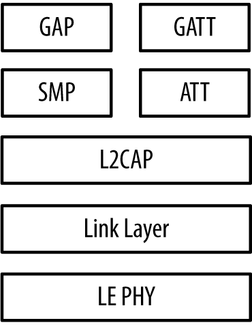
\includegraphics[width=0.3\textwidth]{layers}
    \caption{Bluetooth low energy key exchange protocol}
  \label{fig:layers}
\end{figure}


While BLE has the same top-level layers as Bluetooth Classic (GATT and L2Capp 
layer), it has differences on the low level layers (physical and link layer).

\subsection{Physical layer} \label{ssec:phy}

BLE operates in the same 2.4 GHz frequency band as Bluetooth classic. Though it 
uses only 40 instead of 80 channels where each channel has 2 MHz space. 37 of 
these channels are used for data transmission and 3 channels are for 
advertisement. Devices advertise their services and the ability to connect to 
them on these three channels; connection establishment is also performed on 
these channels. Different from Bluetooth Classic, BLE uses the Gaussian 
Frequency Shift Keying (GFSK) modulation scheme.

\subsubsection{Channel hopping}

To prevent interference with other connections and wireless technologies, BLE 
uses frequency hopping and changes the channel after a defined amount of time. 
The channels are switched according to the following formulae:

\begin{align*}
  %\label{eq:}
  newchannel = currentchannel+hopincrement \% 37
\end{align*}

where advertisment channels are not considerated for simplification. The channel is changed in a defined interval hoptime, i.e.\ every "\emph{hoptime}" milliseconds, the channel is hopped according to the given formulae.

\subsection{Link layer} \label{ssec:link}

\begin{figure}
  \centering
    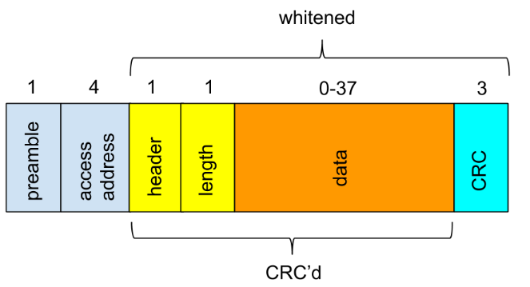
\includegraphics[width=0.5\textwidth]{blepacketformat}
    \caption{Bluetooth low energy packet format \cite{imgsrc:packetformat} }
  \label{fig:packetformat}
\end{figure}

BLE packets are made of the components shown in figure~\ref{fig:packetformat} 
and consist of between 10 and 47 bytes. The first 8 bit are a fixed preamble 
to indictae the packet is a BLE packet. The next 32 bit are the access address. 
For advertising packets, this field always has the value ''0x8E89BED6'', for 
normal 
data packets it is a connection specific value. 

The next field is the 
PDU (Protocol data unit) which contains the actual payload/user data and 
consists of 2-39 bytes dependent on the application layer packet size. In the 
end there is a simple CRC value which functions as a checksum to verify the 
integrity of the package content.
In Bluetooth low energy to keep power consumption low, many mechanisms are less aggressive than on Bluetooth classic. Specificially the hopping rate and the whitening of PDU are simpler and as a result of that as well simpler to eavesdrop.

\subsection{Connection} \label{ssec:con}

As the bluetooth peripheral device sends advertisment packages, the central device, which is often represented by a smartphone-similar device is responsible of detecting and connecting to it. During this connection establishment the two devices setup the connection which includes parameters like \emph{channel hop time} and \emph{channel increment}, but also initialize the encryption, if enabled. After the connection is established, the two devices talk on 37 channels with channel hopping enabled.

It is worth mentioning, that all PDU and CRC data is whitened (by XORing) with 
a LFSR. Though, as the seed is simply the channel number, it doesn't increase 
security/anonymity as it can easily be reversed in an eavesdropping process.

%KOMMENTAR: Wofür steht LFSR? Eine ausgeschriebene Eräuterung wäre hier 
%hilfreich.

\section{Encryption}

BLE uses AES-CCM for it's encryption. This standard ensures data encryption and 
integrity at the same time. It is used in many applications as for example WLAN 
and is considered to be unbroken. It is a public and secure standard - 
analyzing it is beyond the scope of this paper. Though, the key exchange 
protocol used by BLE is another story. The key 
exchange protocol was invented exclusively by the Bluetooth association and is 
broken by design.

%KOMMENTAR: Wofür steht AES-CCM? Eine ausgeschriebene Eräuterung wäre hier 
%hilfreich.

\subsection{Key exchange}
\label{sub:key_exchange}

As mentioned in section~\ref{ssec:con}, encryption starts during connection by exchanging the keys. This is the basis of the encryption and all subsequent keys are based on this first key exchange.

Bluetooth connecting security is established in general, by letting the two 
parties know the same key (the \emph{temporary key}) and after that let them 
proof, that they indeed have the same key to verify them. As they cannot simply 
send the key to each other, as anybody could claim to have the correct key 
then, they compute a so called confirm value to share their knowledge about the 
secret without sharing the temporary key.

\begin{figure}
  \centering
    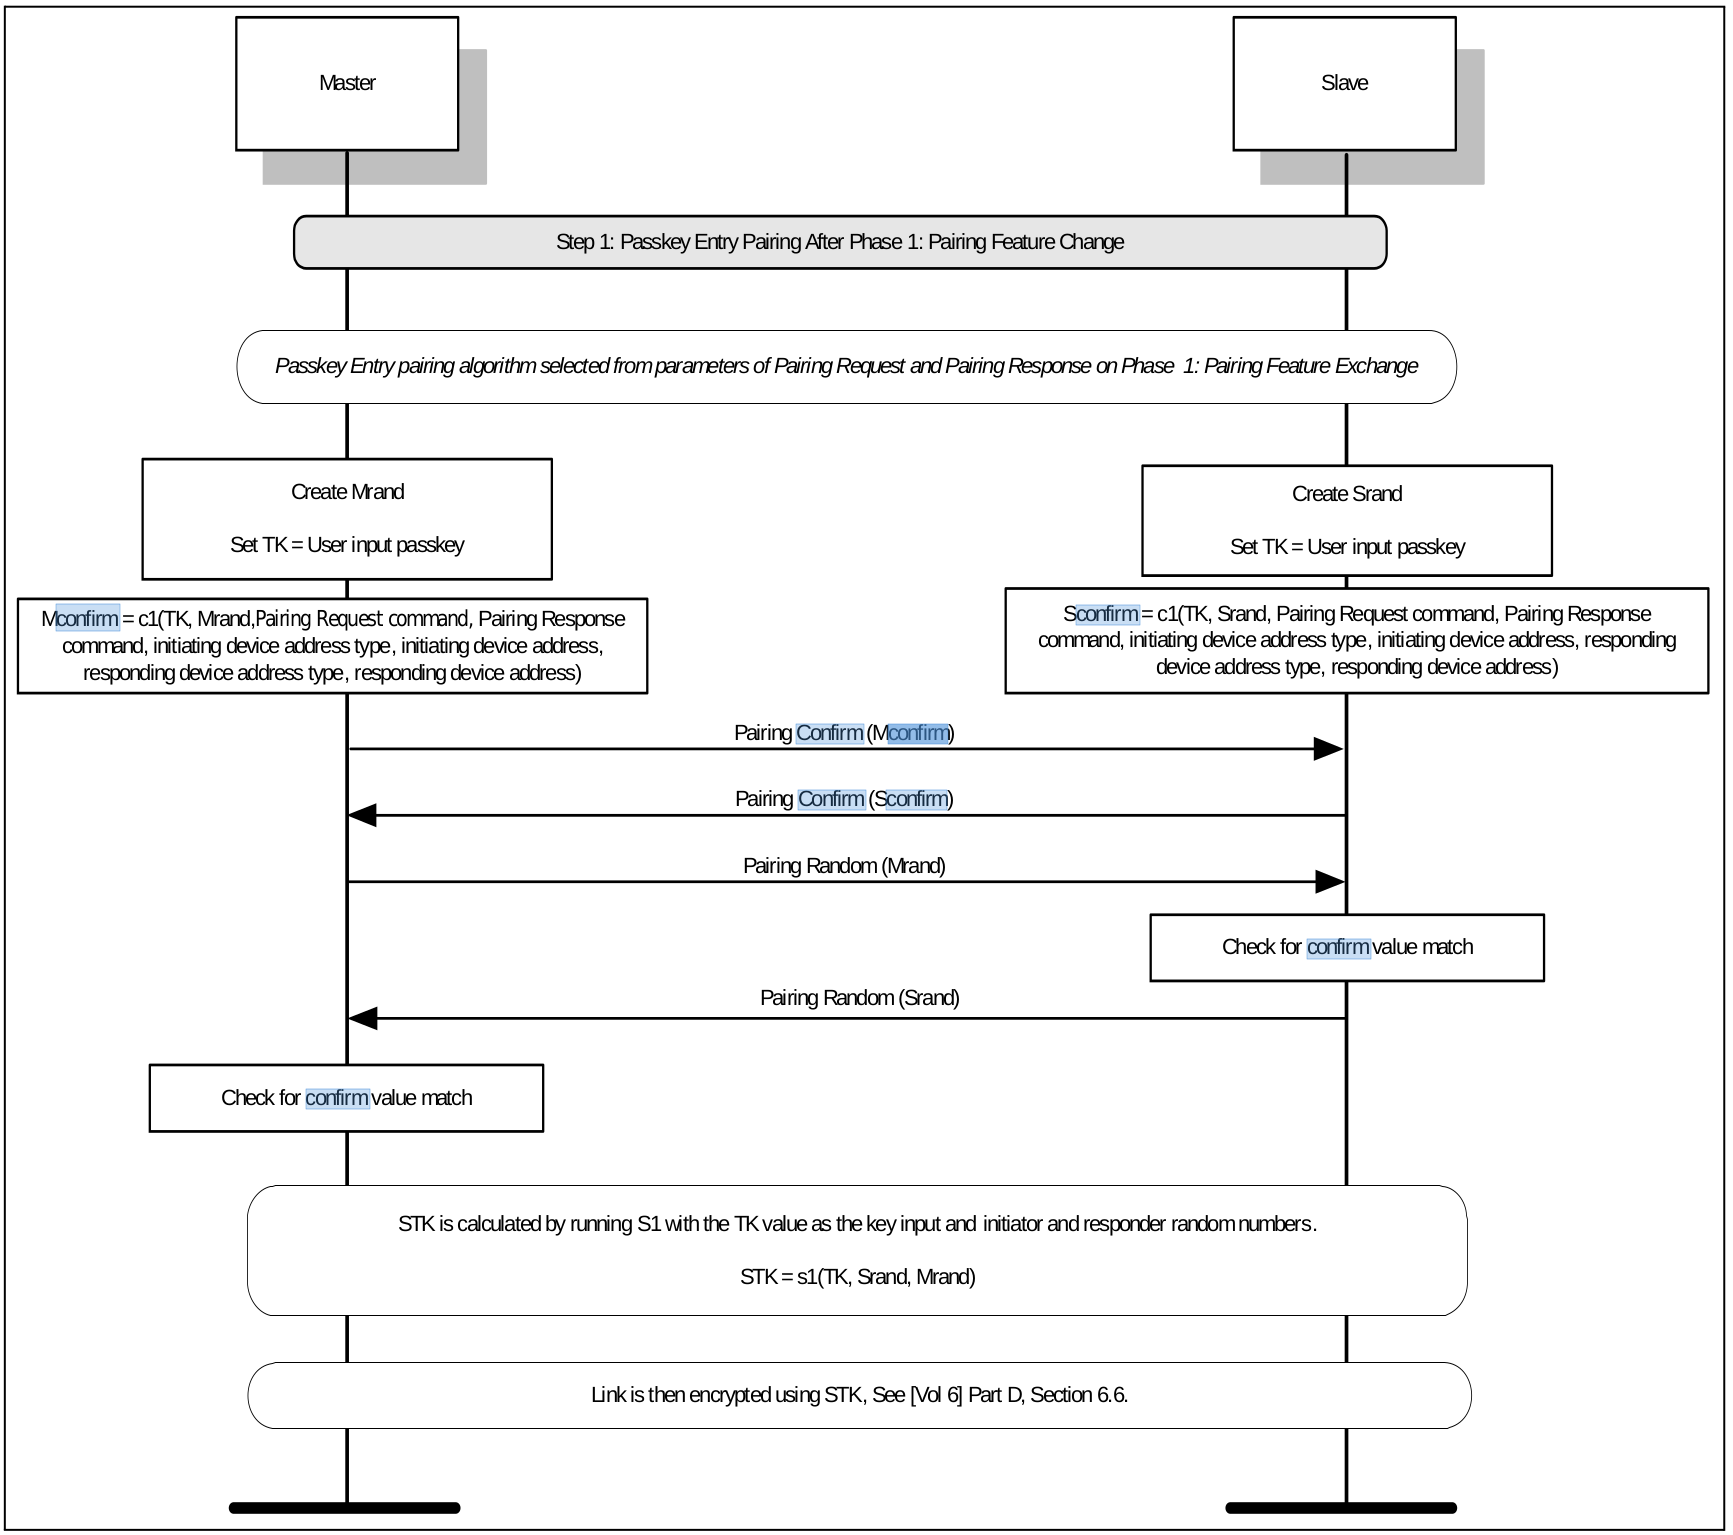
\includegraphics[width=0.5\textwidth]{keyexchange}
    \caption{Bluetooth low energy key exchange protocol \cite{ble40}}
  \label{fig:keyexchange}
\end{figure}

To do so the two parties (M which starts the connection and S who responds to 
the connection attempt) generate one random value each ($rand_M$ and $rand_S$). 
Using these random values, the temporary key and other \emph{known} values such 
as the intiating device address, based on the AES algorithm, they compute so 
called \emph{confirm} values. Which are shared as shown in 
figure~\ref{fig:keyexchange}: M sends S his confirm value $confirm_M$ and S 
sends M his confirm value $confirm_S$. Then, M sends S his random value 
$rand_M$. S now has everything to compute $confirm_M$ and can as such verify if 
M is in the possession of the correct temporary key. If the verification 
succeeds, S sends his random value $rand_S$ to M so M can verify, that S has 
the correct temporary key.

%KOMMENTAR:
%Diesen Part verstehe ich nicht ganz - evtl. könntest du hier nochmal etwas 
%genauer auf den Key Exchange eingehen. Wozu dieser Aufwand? Mir ist nicht ganz 
%klar warum das sicher ist. 

After this procedure is done, both parties know, they are in the possession of the same (correct) temporary key. They compute a series of different keys based on the Temporary Key to finally be able to compute session keys used for the AES encryption of the user data.

\section{Attacks}
\label{attacks}

To attack BLE it is necessary to
\begin{itemize}
  \item detect and interpret (sniff) packages
  \item sniff the key exchange packets in order to crack the encryption keys
\end{itemize}

While it is always possible to eavesdrop unencrypted connections, for encrypted connections there are two scenarios in which a connection would be provably secure:
\begin{itemize}
  \item The connection establishment, and as such the key exchange, is done in a safe, eavesdroppping secured place (for example faraday cage)
  \item The \emph{OOB} pairing mode is used.
\end{itemize}

Although \emph{OOB} pairing mode is indeed safe, it is impractical to use and is in practice never used.

\subsection{Sniffing}

To sniff bluetooth packets, a device is necessary which reads bitstreams on the given frequency band (which is one of the 2.4 GHz channels) by decoding the GFSK modulation. While this is a simple task it involves antennas, radio chips and microcontrollers. The ubertooth project~\cite{ubertooth} implements such a device enabling sniffing on the Bluetooth Low Energy physical layer adaptively (by updating the channel which should be sniffed accordingly). This bit stream may include information from many different connections and/or wireless technologies. To find a bluetooth packet in that bitstream, the \emph{preamble} (see section~\ref{ssec:link}) can be used as a pattern to look for. The upcoming 32-bit form the access address then and show if the packet is interesting or not (is it the connection, the attacker is interested in?). Now the next bits, the PDU and CRC data, are whitenend and as such must be XORed with the an LSFR seeded by the channel number which is sniffed to clear the whitening of the data. At this point the packet is successfully restored on the link layer.
% Maybe add the fact that there are many rubbish packets?

%KOMMENTAR: Wofür steht GFSK? Eine ausgeschriebene Eräuterung wäre hier 
%hilfreich.

%(is it the connection, the attacker is interested in?) -> was ist das?
%are whitenend and as such must be XORed with the an LSFR seeded by the channel 

%number which is sniffed to clear the whitening of the data. -> zu viele 
%unklare Abkürzungen

In practice it is most convenient to sniff on the three advertisement channels: 
The connection establishment can be seen and all parameters necessary to follow 
and decrypt a connection can be recovered. As the hop-interval and 
hop-increment are done by the connection establishment, it is possible to 
change the sniffed channel according to that scheme to follow and decrypt the 
complete connection.

\subsection{Connection reset} \label{ssec:conreset}

Often it is the case, that a connection has already been established and it is not possible to sniff the connection parameters in order to follow the connection. In that case it is possible to provoke a connection reset which leads to another connection establishment.
To provoke a connection reset, packet injection has to be done. Looking at section~\ref{ssec:phy} and~\ref{ssec:link} we see what has to be done to generate and inject a packet, given the payload, that is intended to be sent:

\begin{enumerate}
  \item Generate PDU header
  \item Generate CRC (based on PDU content)
  \item Whiten data (use LSFR)
  \item Generate full package by prepending access address and preamble
  \item Send out on phy layer on the appropriate band using GFSK (e.g.\ use ubertooth)
\end{enumerate}

The BLE reference shows the structure of packets to provoke disconnection and 
connection reset on pages 564 and 64 (Section 4.6 DISCONNECTION REQUEST (CODE 
0x06)) and show which PDU data has to be used to provoke the connection reset 
which will lead to a new connection establishment. \cite[p. 564]{ble40}

\subsection{Channel following}
\label{channelfollowing}

Section~\ref{ssec:conreset} is a proper way to provoke a new connection establishment in order to sniff connection parameters which enable us to follow a communcation through all the channels. As it might be desirable to attack passively, such that no-one can detect the existent of an attacker, that attack is not ideal, as it injects packets. Though, there is a way to follow an ongoing connection by calculating the necessary hop-interval and hop-increment values, which is completely passive. Based on the fact, that the number of (data-)channels is a prime(37), we know that all channels will be used once before the first one is used again.

\begin{figure}
  \centering
    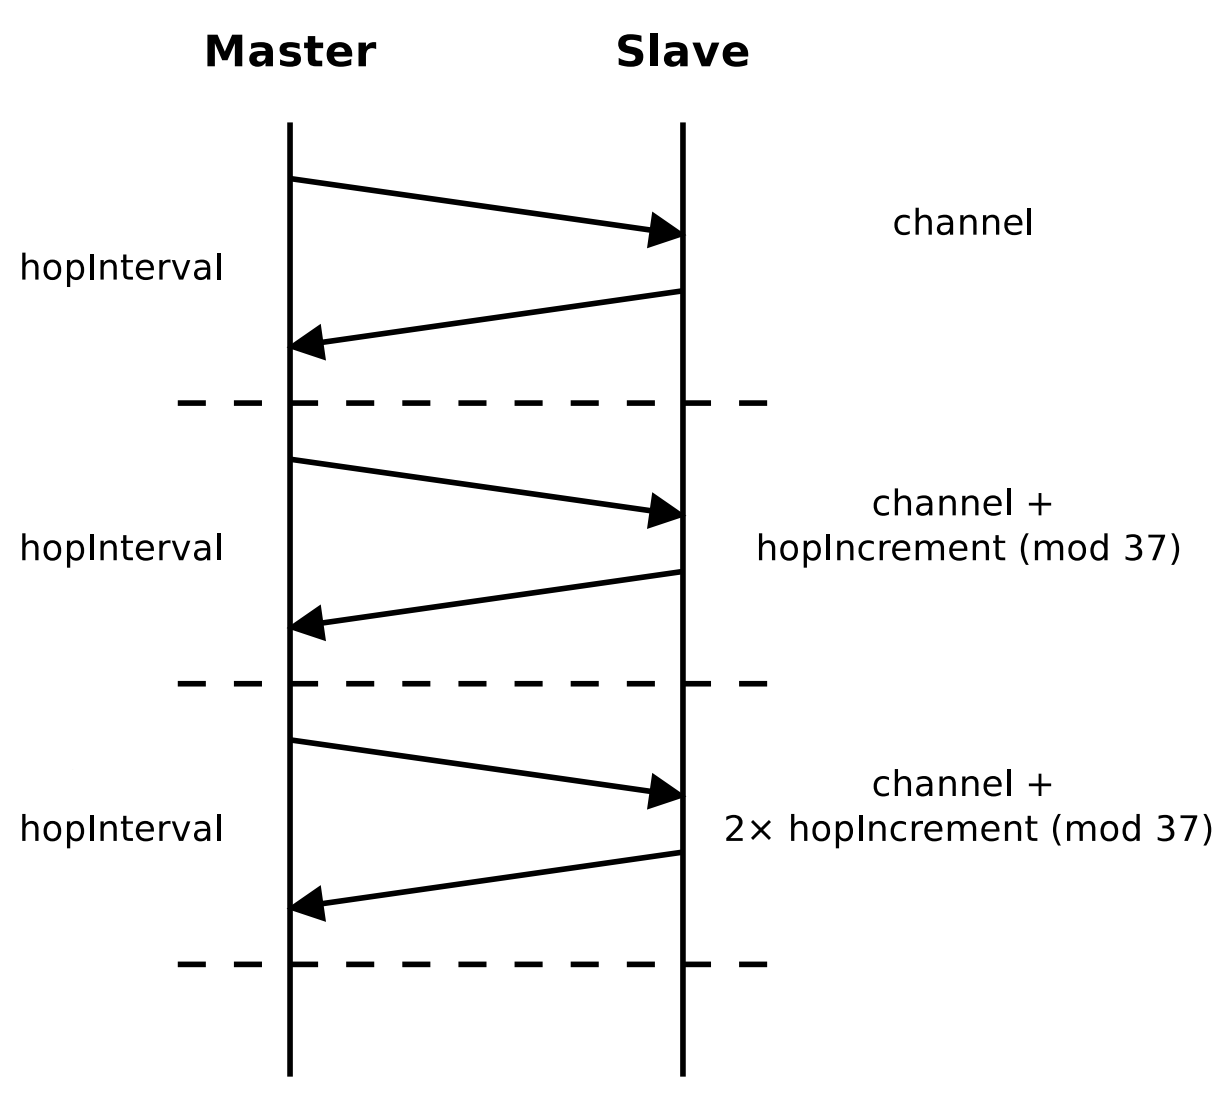
\includegraphics[width=0.5\textwidth]{hopping}
    \caption{BLE Hopping scheme \cite{lowenergylowsecurity} }
  \label{fig:hopping}
\end{figure}

\subsubsection{Hop interval}
\label{ssub:hop_interval}

As such we can look for an established connection (using preamble and access address) detect, when it sends packages at a certain channel once and wait for it to send data again on that channel. The time difference can be divided by 37 to get the hop-interval (the time, the connection resides on a channel before hopping to the next):

\begin{equation*}
  hopinterval = \frac{\Delta t}{37}
\end{equation*}

\subsubsection{Hop increment}
\label{ssub:hop_increment}

Calculating the hop-increment involves a bit more math. To gather the necessary 
information, we listen first on channel 0, hop to channel 1 and wait to receive 
a package from the desired connection. Knowing the hop-interval already, we 
know how many hops the connection has performed before reaching channel 1. By 
knowing the number of hops that were performed we can generate a lookup-table 
by using Fermat’s little theorem or simple by brute-forcing all combinations to 
find a mapping from hop-count to \emph{hop increment}. Once these two values 
(hop interval and increment) are known, we can follow the connection in order 
to capture the full transmitted data.

\subsection{Key breaking}

As described in section~\ref{sub:key_exchange} the two parties establishing a 
connection exchange (in plaintext) several values to ensure they have the same 
temporary key. The key in cracking the temporary key is the confirm value.

\begin{equation*}
  \begin{split}
  confirm = c1 ( TK , \\Mrand , \\Pairing \\Request command, \\Pairing Response command, \\initiating device address type, \\initiating device address, \\responding device address type, \\responding devices address)
  \end{split}
\end{equation*}

c1 is a function based on AES which provides one-wayness.
Looking at the equation, we can analyze which of the fields we know as an attacker (as they were transmitted in plaintext over the air). Namely:

\begin{itemize}
  \item Confirm
  \item Rand
  \item Pairing Request command
  \item Pairing Respond command
  \item initiating device address type
  \item initiating device address
  \item responding device address type
  \item responding device address
\end{itemize}

In fact, the only value, we don't know in this formulae, is the temporary key TK. As told in the specification, in the most of the cases, TK is either 0 or a value between 0 and 999999. This numbers are too small to defend against a simple bruteforce attack and as such it is possible to try out all different values of TK, calculating the corresponding confirm value and compairing it with the sniffed one. Having found the TK that leads to a matching confirm value gives us the possibility to calculate the different keys defined in the specification to end up with the session key which gives us the ability to decrypt the entire transmission.

\section{Key exchange protocol in 4.2}

To prevent man-in-the middle attacks and passive eavesdropping as described in section~\ref{attacks}. To do so, the specification introduces the Elliptic curve Diffie–Hellman (ECDH) algorithm for key generation. The algorithm enables proper asymetric encryption to share a key without caring about evesdropers.


% needed in second column of first page if using \IEEEpubid
%\IEEEpubidadjcol

% An example of a floating figure using the graphicx package.
% Note that \label must occur AFTER (or within) \caption.
% For figures, \caption should occur after the \includegraphics.
% Note that IEEEtran v1.7 and later has special internal code that
% is designed to preserve the operation of \label within \caption
% even when the captionsoff option is in effect. However, because
% of issues like this, it may be the safest practice to put all your
% \label just after \caption rather than within \caption{}.
%
% Reminder: the "draftcls" or "draftclsnofoot", not "draft", class
% option should be used if it is desired that the figures are to be
% displayed while in draft mode.
%
%\begin{figure}[!t]
%\centering
%\includegraphics[width=2.5in]{myfigure}
% where an .eps filename suffix will be assumed under latex,
% and a .pdf suffix will be assumed for pdflatex; or what has been declared
% via \DeclareGraphicsExtensions.
%\caption{Simulation Results}
%\label{fig_sim}
%\end{figure}

% Note that IEEE typically puts floats only at the top, even when this
% results in a large percentage of a column being occupied by floats.


% An example of a double column floating figure using two subfigures.
% (The subfig.sty package must be loaded for this to work.)
% The subfigure \label commands are set within each subfloat command, the
% \label for the overall figure must come after \caption.
% \hfil must be used as a separator to get equal spacing.
% The subfigure.sty package works much the same way, except \subfigure is
% used instead of \subfloat.
%
%\begin{figure*}[!t]
%\centerline{\subfloat[Case I]\includegraphics[width=2.5in]{subfigcase1}%
%\label{fig_first_case}}
%\hfil
%\subfloat[Case II]{\includegraphics[width=2.5in]{subfigcase2}%
%\label{fig_second_case}}}
%\caption{Simulation results}
%\label{fig_sim}
%\end{figure*}
%
% Note that often IEEE papers with subfigures do not employ subfigure
% captions (using the optional argument to \subfloat), but instead will
% reference/describe all of them (a), (b), etc., within the main caption.


% An example of a floating table. Note that, for IEEE style tables, the
% \caption command should come BEFORE the table. Table text will default to
% \footnotesize as IEEE normally uses this smaller font for tables.
% The \label must come after \caption as always.
%
%\begin{table}[!t]
%% increase table row spacing, adjust to taste
%\renewcommand{\arraystretch}{1.3}
% if using array.sty, it might be a good idea to tweak the value of
% \extrarowheight as needed to properly center the text within the cells
%\caption{An Example of a Table}
%\label{table_example}
%\centering
%% Some packages, such as MDW tools, offer better commands for making tables
%% than the plain LaTeX2e tabular which is used here.
%\begin{tabular}{|c||c|}
%\hline
%One & Two\\
%\hline
%Three & Four\\
%\hline
%\end{tabular}
%\end{table}


% Note that IEEE does not put floats in the very first column - or typically
% anywhere on the first page for that matter. Also, in-text middle ("here")
% positioning is not used. Most IEEE journals use top floats exclusively.
% Note that, LaTeX2e, unlike IEEE journals, places footnotes above bottom
% floats. This can be corrected via the \fnbelowfloat command of the
% stfloats package.



\section{Conclusion}
Bluetooth low energy in specification versions 4.0 and 4.1 is broken by design. 
Not only is it possible to track and eavesdrop ongoing connections, but also 
the key exchange protocol is broken in these versions resulting in millions of 
insecure connections nowadays. Tools to apply the known attacks are available 
in the Internet. Future devices can be based on the new standard 4.2, which 
supports a secure key exchange protocol. Though many devices from nowadays 
will not get updates.


% if have a single appendix:
%\appendix[Proof of the Zonklar Equations]
% or
%\appendix  % for no appendix heading
% do not use \section anymore after \appendix, only \section*
% is possibly needed

% use appendices with more than one appendix
% then use \section to start each appendix
% you must declare a \section before using any
% \subsection or using \label (\appendices by itself
% starts a section numbered zero.)
%


\appendices
\section{Proof of the prime number channel hop circle completeness}

In section~\ref{channelfollowing} we refered to the fact that independently 
from the chosen hop increment all channels will be used once after the same 
channel will be used a second time. We will proof this simple fact in this 
section.

To proof this we assume the opposite: There is a hopincrement (which is no multiple of 37) which reaches its start channels again, before it hopped over all 37 channels:

\begin{equation*}
  \exists x\in\mathbb{N}\setminus (\mathbb{N} * 37), \exists n\in\mathbb{N}\ldotp x*n \% 37 = 0 \wedge n < 37
\end{equation*}
which is the same as
\begin{equation*}
  \begin{split}
    \exists x\in\mathbb{N}\setminus (\mathbb{N} * 37), \exists n\in\mathbb{N}\exists y\in\mathbb{N}\ldotp x*n = 37 * y \\
    \exists x\in\mathbb{N}\setminus (\mathbb{N} * 37), \exists n\in\mathbb{N}\exists y\in\mathbb{N}\ldotp \frac{x*n}{y} = 37
  \end{split}
\end{equation*}

As we see, to get $37$ on the right side either $x$ or $n$ must be a multiple of $37$, because $y$ is in $\mathbb{N}$ and can't be $\frac{1}{37}$. As $x$ cannot be a multiple of $37$ by definition, $n$ has to be. As such our assumption is wrong and we can conclude:

\begin{equation*}
  \forall x\in\mathbb{N}\setminus (\mathbb{N} * 37), \forall n\in\mathbb{N}\ldotp x*n \% 37 = 0 \wedge n = \mathbb{N} * 37
\end{equation*}

This proof holds for any prime number. We just used 37 to show it specificially for the channel hopping case.

% use section* for acknowledgement
\section*{Acknowledgment}

The author would like to thank Mike Ryan for his great work on Bluetooth Low Energy Sniffing and Security Research.

% Can use something like this to put references on a page
% by themselves when using endfloat and the captionsoff option.
\ifCLASSOPTIONcaptionsoff
  \newpage
\fi



% trigger a \newpage just before the given reference
% number - used to balance the columns on the last page
% adjust value as needed - may need to be readjusted if
% the document is modified later
%\IEEEtriggeratref{8}
% The "triggered" command can be changed if desired:
%\IEEEtriggercmd{\enlargethispage{-5in}}

% references section

% can use a bibliography generated by BibTeX as a .bbl file
% BibTeX documentation can be easily obtained at:
% http://www.ctan.org/tex-archive/biblio/bibtex/contrib/doc/
% The IEEEtran BibTeX style support page is at:
% http://www.michaelshell.org/tex/ieeetran/bibtex/
%\bibliographystyle{IEEEtran}
\bibliographystyle{ieeetr}
% argument is your BibTeX string definitions and bibliography database(s)
%\bibliography{IEEEabrv,../IEEEtran}
\bibliography{main}
%
% <OR> manually copy in the resultant .bbl file
% set second argument of \begin to the number of references
% (used to reserve space for the reference number labels box)

% biography section
%
% If you have an EPS/PDF photo (graphicx package needed) extra braces are
% needed around the contents of the optional argument to biography to prevent
% the LaTeX parser from getting confused when it sees the complicated
% \includegraphics command within an optional argument. (You could create
% your own custom macro containing the \includegraphics command to make things
% simpler here.)
%\begin{biography}[{\includegraphics[width=1in,height=1.25in,clip,keepaspectratio]{mshell}}]{Michael Shell}
% or if you just want to reserve a space for a photo:

% \begin{IEEEbiography}[{\includegraphics[width=1in,height=1.25in,clip,keepaspectratio]{picture}}]{John Doe}
% \blindtext
% \end{IEEEbiography}

% You can push biographies down or up by placing
% a \vfill before or after them. The appropriate
% use of \vfill depends on what kind of text is
% on the last page and whether or not the columns
% are being equalized.

%\vfill

% Can be used to pull up biographies so that the bottom of the last one
% is flush with the other column.
%\enlargethispage{-5in}




% that's all folks
\end{document}



